\chapter{引言}
\label{cha:intro}

\section{研究背景与意义}

情感识别旨在了解人们对特定事件或实体的态度和情感。自Web2.0普及后,大量网民每天在互联网生产着各种各样的内容,其中包含不同方面的信息,如个人生活经历,购买行为,对产品服务的体验评价,对社会时事的看法等等。从人们的日常社交需求来看,这种借由互联网媒体的分享非常便捷,我们可以了解到亲朋好友的近况,也可以和不认识的网民交流对具体事件的想法。在商业上,借由对用户的网络行为进行分析,企业可以对他们的客户或者潜在客户有更深入的了解,对他们的需求和反馈及时作出反应将带来战略性的优势。在社会管理上,政府可以透过对网民在网络上的发言了解人民的想法和舆论的走向,进而作出相应的措施。正因为互联网的普及,才使得以上基于对特定人群的了解来进行决策的做法成为可能。随着数据资源变得丰富,相应的技术在近年得以快速发展,目前市面上已经有公司(如国内的腾讯和阿里巴巴,以及国外的微软和亚马逊等)提供基于大型社交媒体平台(如微博、讨论区等)上的数据进行情感分析相关的规泛化服务,然而相应的技术依然有进步空间,研究工作还在不同方向上摸索。

情感在人们的思想表达和交流中起着重要作用\cite{Banerjee2015Detection},比起了解该想法的细节内容,情感对应该想法的一种倾向。譬如在分析用户对新产品的评论时,
只需要分析其中褒贬意思的倾向即可大致了解新产品是否能让大部分的客户满意,或者筛选出其中表示不满意的用户再进行深入分析,因此情感识别技术具有一定的应用价值。而由于在互联网上,大部分情况下用户以文本表达想法,面向文本的情感识别成为了近年最重要的研究课题之一。相对于人们面对面交流的场景,聆听者可以根据发言者的肢体语言、面部表情以及声调变化等额外信息更好地理解发言者想表达的意思,然而这些信息并不存在于文本当中,这也正是对文本进行情感识别本身的难点之一\cite{SemEval2019Task3}。

情感识别的另一个难点在于语言中丰富多样的修辞手法,其中反讽是具代表性的修辞手法之一。Henry Watson Fowler在《The King's English》一书中描述“即使对反讽的定义有数百种, 其中只有包含'表面意思和实际意思不同'这个概念的才能被接受”。Eric Partridge 在《Usage and Abusage》一书中指出“反讽存在于所表达意思的另一面”。总的多说当反讽在文本中出现,那么发言者想表达的意思应该和文本的字面意思完全相反。譬如某人表示“我就喜欢你不断挑战我的底线”,在字面上“喜欢”表达的是正面的情感,然而根据常识可知“挑战底线”是一种让人反感的行为,与“喜欢”相矛盾。这段文字实则表示发言者正被某人触及底线,表达的是负面情感。所以在情感识别当中,正确识别出反讽的使用能够避免对内容的错误理解,反讽识别因此成为了和情感识别紧密相关的研究课题。

\section{国内外研究现状}

\subsection{情感模型}

情感计算的基础是对情感作出描述,现有的描述方式可以分成两个大类: 范畴观和维度观。范畴观即把不同情感对应到一组离散的情感标签上,其中具代表性的有Plutchik的情感模型\cite{Plutchik1980Emo}和Ekan的情感理论\cite{Ekman1992An}。Plutchik的情感模型包含八种情感:愤怒、恐惧、悲伤、厌恶、期待、信任、高兴、惊讶;这些情感都各自对应具有重要生存意义的行为,各种复杂的情感都是由这此基本情感构成,另外这八种情感可以分成四组对立的情感对。Ekan在十年后提出的情感理论和Plutchik的相似,但相对地少了期待和信任两种情感,是一个六类情感模型。

\begin{figure}[h]
  \centering%
  \subcaptionbox{三维模型\label{fig:plutchik_emotion_wheel_3d}} %[3cm] 标题的长度,超过则会换行,如下一个小图。
    {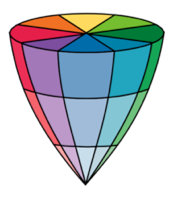
\includegraphics[height=4cm]{img/plutchik_3d.png}}%
  \hspace{4em}%
  \subcaptionbox{二维模型\label{fig:plutchik_emotion_wheel_2d}}
      {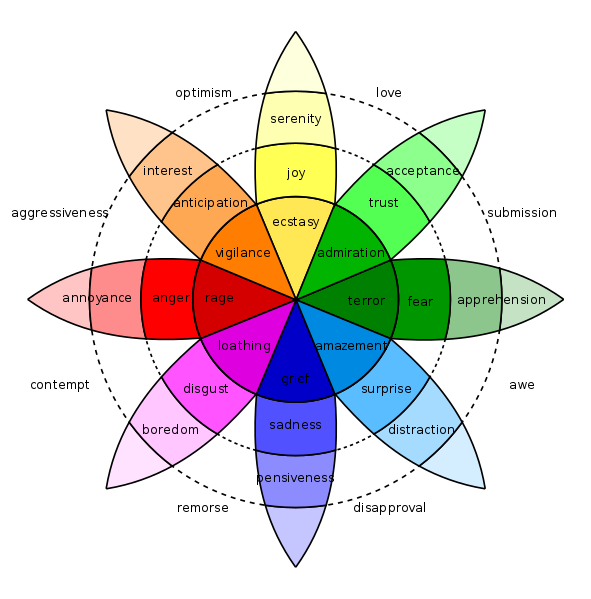
\includegraphics[height=8cm]{img/plutchik_2d.png}}
  \caption{Plutchik\cite{Plutchik1980Emo}提出的情感轮模型}
  \label{fig:plutchik_emotion_wheel}
\end{figure}

以维度观描述情感就是把情感映射到多维空间的点上,而目前维度观情感模型以二维和三维空间的为主。二维情感模型中较有代表性的是Russell提出的环状模型(Circumplex Model)\cite{Russell1980Cir} ,其中纵坐标对应情感的激活度(Arousal),横坐标对应情感向性(Valence),而不同的情感则分布在一个环状的区域内。Bradley等人\cite{Bradley1992Rem}提出的向量模型(Vector Model)在对横轴和纵轴的定义和前者相似,但其理论假设高激活度的情感应该有较明显的正负倾向,相对地低激活度的情感则偏向中性,故情感分布在一个回力标形状的区域。Watson和Tellegen \cite{Watson1985Tow} 提出的 PANA(positive activiation-negative activation)模型和前两者在理论基础上则有明显的不同,他们认为情感的正面作面和负面作用是两个独立的成分,所以在模型中纵轴和横轴分别表示情感正面作用和负面作用的强弱,不过该模型相当于把Russell等人提出的环状模型的向量空间旋转45度\cite{Rubin2009A}。

基于三维空间的情感模型中具有代表性的有Plutchik\cite{Plutchik1980Emo}提出的情感轮模型,Plutchik认为情绪之间包含强度,相似性和两极性三种维度,椎体的顶部和底部分别对应强的情感和弱的情感,相似的情感对应椎体中相近的位置,对立的的情绪则会对应到椎体中对立的位置上。另外还有Mehrabian \cite{Mehrabian1996Pleasure}提出的PAD模型,其三维空间的三个坐标轴分别对应情感愉悦度(Pleasure)、激活度(Arousal)以及优势度(Dominance)。较近期被提出的是Hugo\cite{Hugo2012A}的情感立方体模型,其三维空间的三个坐标轴分别对应5-羟色胺(5-hydroxytryptamine, 5-HT), 多巴胺(dopamine,DA)和去甲肾上腺素(noradrenaline,NE)三种神经递质所产生信号的强弱,并对空间中一个立方体的八个顶点标记了其对应的情感。

\begin{figure}[H] % use float package if you want it here
  \centering
  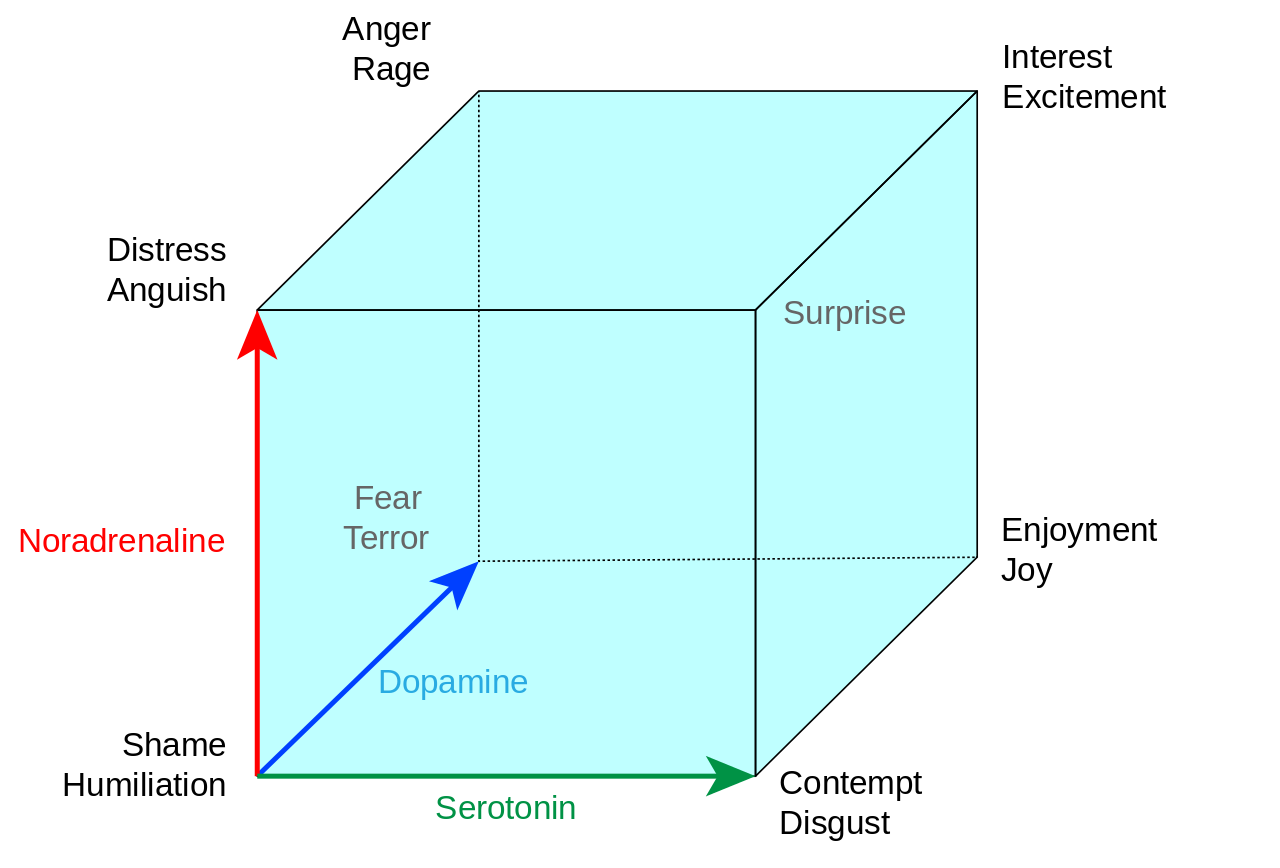
\includegraphics[width=0.8\textwidth]{img/hugo_cube_of_emotion.png}
  \caption{Hugo\cite{Hugo2012A}提出的情感立方体模型}
  \label{fig:hugo_cube_of_emotion}
\end{figure}

\subsection{情感识别}

对应上述情感模型的分类,情感识别研究可以分成两类。第一类对应范畴观,给定一组情感类型,判断一段文本中所表达的情感倾向于该组情感中的哪一种,或者是否包含这一组情感中的一种或多种情感。如国际比赛SemEval-2018任务一\cite{mohammad2018semeval}的子任务要求识别一段微博中是否包含愤怒、恐惧、悲伤等十一种情感中的一种或多种情感。另一类情感识别研究对应维度观,对于给定的情感属性,判断一段文本中该情感属性的强度。其中常见的有情感向性的二分类问题(正性或负性)、三分类问题(正性、中性或负性)、五分类问题(非常正性,正性、中性、负性或非常负性)。其中五分类问题的研究对象一般是互联网上五星评分制的产品评论或者电影评论等。

另一方面,目前文本情感识别的研究按照文本的粒度可以大致分成三类:文章级别、句子级别、属性级别。在文章级别的情感识别中,虽然一篇文章由多个句子组成,但假设整篇文章存在某种情感倾向,而研究目标则是自动识别出该种情感倾向的类型或强度。Turney \cite{turney2002thumbs} 利用线上电影评论中"推荐"(大拇指朝上)和"不推荐"(大拇指朝下)的标记研究对电影评论的正负性情感识别。他提出利用点互信息(Pointwise Mutual Information,PMI)来评估单词的语义倾向性,其中PMI透过在大型语料库中统计两个单词共同出现的情况来评估两个单词的相似度。首先利用PMI值评估各个单词与正向情感的代表性单词"excellent"和负向情感的代表性单词"poor"的相似性,再取这两个PMI值作差得出该单词在语义上倾向于哪一种情感,再透过计算整段评论的平均语义倾向性评估整体的情感倾向。Pang和Lee \cite{pang2004sentimental} 采用了不同的方法研究相同的问题。他们首先对评论中每个句子的主观程度进行评分,利用评分构造一个带权重的句子关系图,再基于最小割算法结合上下文加强对每个句子主观程度的判断,过滤评论中不带主观情感的句子后再判断整个评论的情感向性,以此加强识别效果。Tang等人 \cite{tang2015learning} 则研究了产品评论的五级评分预测。除了评论的文本内容,他们进一步引入了用户的信息和产品的信息。经过数据分析,他们发现相同用户对不同产品的评论和评分比不同用户之间的更一致,另外不同用户对同一产品的评论和评分比不同产品之间的更一致,这显示了用户和产品各自都存在一些相对固定的属性。因此Tang等人提出一种为用户和产品生成表示向量的方法,并应用于评论的五级评分预测。实验结果显示他们的方法在多个数据集上达到了较好的性能,这同时引出了加入背景信息来加强系统识别能力的可能性。

然而一篇文章有可能同时表达了多种观点和情感,因此有另一类研究针对句子或短文本所表达的情感,即句子级别的情感识别。由于句子的文本长度较文章的短,文本内部的逻辑较简单,但相对地所包含的提示信息也较少,课题的难点与前者有所不同。Khan等人\cite{khan2011sentiment}研究了对线上评论中句子进行正负性情感识别。他们首先区分出评论中各个句子的主观性和客观性,然后针对带主观情感的句子,利用开源自然语言工具SentiWordNet获取各个单词的正负情感属性,再根据句子的词性标注和他们设计的规则计算整个句子的情感向性。Khan等人默认单词的正负情感属性在不同场景下不变,然而Li等人\cite{li2013constructing}指出部分单词在特定场景下会有不同的情感向性,因此他们提出了一种有监督学习方法,自动学习各单词在指定领域下的情感向性,以此作为文本的特征,并应用于对产品评论的情感识别中。实验结果显示使用SentiWordNet提供的全局情感评分和针对领域评估的情感评分相比,使用后者能达到的识别性能力更好,验证了他们的假设。一些研究则选择端到端地学习单词的情感和语义倾向,在Santos和Gatti\cite{dos2014deep}对电影评论和微博的情感识别研究中,他们提出了利用卷积神经网络分别从字符级别和词级别计算出单词对应的特征向量,然后同样以卷积神经网络结合句子中各单词的向量得出句子的表示向量和预测整体的情感倾向。结果显示他们的方法较早期的其他方法性能更好。

在一些应用场景当中,我们希望了解发言者对某个对象或者它的某个特定属性的想法。譬如新手机推出市场后,厂商需要了解用户对手机的续航能力、拍照质量、交互体验等各方面的评价,那么对于评论中同时谈论手机的多个属性且好评和差评不一时,应该针对各个属性分别识别发言者所表达的感情,因此有了属性级别的情感识别。Che等人\cite{che2015sentence}提出一种句子压缩算法,透过对句子进行依存句法分析,过滤与目标属性的情感无关的内容。他们采用了多种语义和语法特征作为输入,以条件随机场(Conditional random field,CRF)作为分类器。实验结果显示过滤掉不相关的文本部分后,识别性能有所提升。Wang等人\cite{wang2016attention}研究了对网上评论中特定实体或属性的情感识别。他们提出了一个基于注意力机制的长短时记忆网络(Long Short-Term Memory,LSTM),特点在于只以词向量作为输入,而不采用其他传统的语义和语法特征,另外利用注意力机制自动识别与目标相关的内容。他们的实验基于国际比赛SemEval-2014任务四\cite{pontiki2014semeval}中的一个子任务,结果然显示他们的系统性能达到了当时的技术水平。另外透过对注意力单元的输出进行分析,验证了注意力机制能够有效识别文本中与目标相关的内容。Tang等人\cite{tang2016aspect}分别对前述数据集中电脑和餐庁相关的两组样本进行属性级别的情感识别,但有别于当时主流的以特征提取为主的浅层机器学习方法(如支持向量机)和针对序列的深度学习模型(如递归神经网络),他们提出了一个基于注意力机制的深度记忆网络。另外针对文本中各个单词和目标单词在句子中的距离,作者引入了距离信息提出了注意力单元的多种变形。实验结果显示他们提出的深度记忆网络达到了当时第一名参赛系统(基于手工特征和支持向量机的算法)的性能。另外对注意力单元的中间结果进行人工分析,验证了在同一段评论中,引入距离信息的注意力单元有助于区分不同单词对不同目标的情感的贡献。

\subsection{反讽识别}

正如前面所述,反讽识别和情感识别紧密相关,识别出反讽的使用对正确识别情感起着关键作用。Tsur等人\cite{tsur2010icwsm}\cite{davidov2010semi}研究了对微博平台Twitter上的微博以及电商平台亚马逊上的评论进行反讽强度的识别,从明显不含反讽到明显表示反讽分成五级,由人工进行标注。他们提出的SASI算法分别从文本提取了词频相关的模式特征以及基于标点符号的特征,以K最近邻算法作为分类器。另外利用在Twitter按井号标签\#sarcastic自动爬取了额外的反讽语料用于初步的模型训练。对实验结果的比较证明了各种特征的有效性以及添加额外语料对模型训练的帮助。

为了以较低成本获取大量的反讽相关语料,很多研究从微博平台根据井号标签自动筛选出可能带反讽的微博。Reyes等人 \cite{reyes2013multidimensional} 利用\#irony,\#education, \#humor, \#politics在Twitter上自动获取四组不同主题的微博,并把\#irony对应的微博和另外三组微博两两组合进行二分类实验。他们提出了四个方面的文本特征提取方法,包括:特殊标记(词汇和标点符号等)、不可预期性、表达风格、情感特性;并比较了每项特征在各组微博中的出现情况,显示了各项特征和反讽的相关性。另外分别采用朴素贝叶斯和决策树作为分类器,但没有明显的性能区别。

类似的数据收集方法对其他语言同样适用。Kunneman等人\cite{kunneman2015signaling}则利用对应的德语井号标签来获取反讽语料,以此研究德语微博中的反讽识别。他们取N元语法作为输入特征,以Balanced Winnow \cite{littlestone1988learning}作为分类器,在测试集上达到约0.85的召回率和0.87的AUC值。但他们进一步经过人工检验评估了基于井号标签自动标注的有效性,分析结果显示该方法获取的反讽样本中包含约10\%的躁声。

\begin{figure}[H] % use float package if you want it here
  \centering
  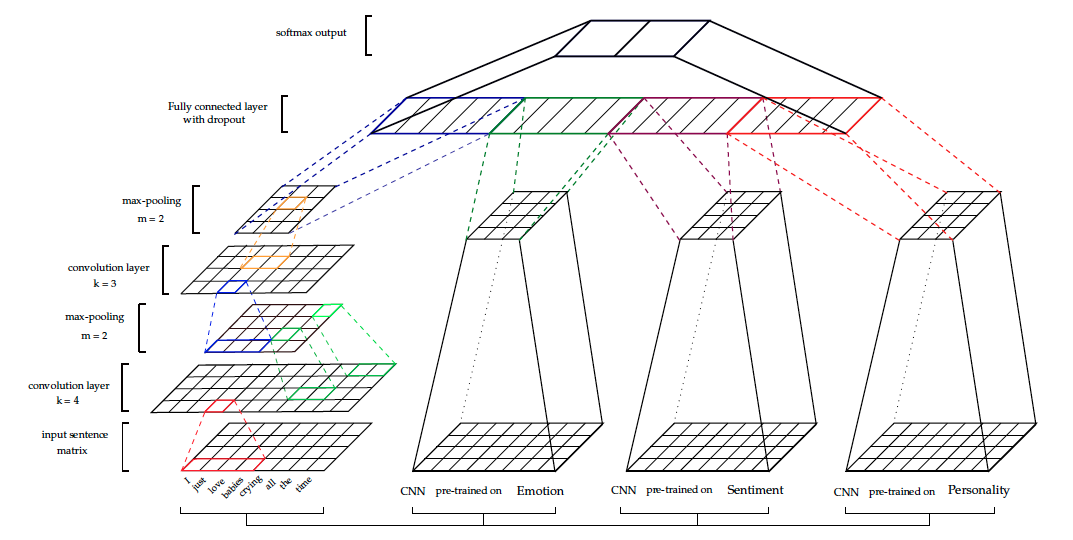
\includegraphics[width=\textwidth]{img/poria2016deeper.png}
  \caption{引入多个领域信息的反讽识别神经网络模型,引自\cite{poria2016deeper}}
  \label{fig:poria2016deeper}
\end{figure}

有别于早期以手动设计的特征作为输入和以传统机器学习方法建模,Poria等人 \cite{poria2016deeper} 首次将神经网络应用于对微博的反讽识别。他们的算法框架主要包含四个卷积神经网络,并分别利用不同的数据集进行预训练,分别对应反讽识别、情感极性识别、情感类型识别和性格识别。最后取四个卷积神经网络的中间结果作为特征,利用支持向量机(Support Vector Machine, SVM)进行后融后得出最终预测结果。实验显示引入反讽识别以外的三个语料库提升了系统的识别能力。

\subsection{社交媒体上的文本情感识别}

随着社交媒体的普及,网民们习惯于在微博、讨论区等平台上表达个人意见和互相讨论。有别于新闻或学术材料等较正式的文件,网民可以较随心所欲地发言,社交媒体因此成为了情感识别的重要研究对象之一。但和产品评论或文章等文本类型不同,社交媒体上的文本普遍较短\cite{Madhusudhanan2018survey},缺少对背景信息的提示,难以判断其内容所属的主题,这对正确理解其中表达的意思带来困难。另外语言中夹杂着不正规的用法,在中文微博中会出现新的短语或对旧短语有新的解释\cite{xie2012jiyu},如“锦鲤”暗示“好运”,“灌水”表示发表没有意义的内容,在英文微博则中会出现错拼字、非正式缩略语、表情符\cite{go2009twitter}\cite{paltoglou2012twitter},如“tnx”对应英文单词“thanks”,“:)”表示微笑等。虽然没有正式的语言组织对这些新的用法进行整合,但因为这些新用法更方便或对思想的表达更丰富到位,随着在网络上的传播而在网民之间达成了共识。传统的文本特征提取建立在标准的单词使用和正规的语法结构上,而由于新词汇和新语用的出现,导致词汇的意思无法被识别或被错误理解,这对于由人工智能理解文本内容成为了一大难点。因此有别于传统的文本研究,在面向社交媒体的文本情感识别时,需要采用额外手段对文本进行预处理,或透过大量语料尝试自动学习这些新出现的语言属性。

Khan等人\cite{khan2014tom}研究了微博的正负中性情感识别。他们提出了一个混合三个分类器的情感识别框架来解决数据稀疏的问题,另外还提出了一组针对微博文本的预处理步骤,其中包括俚语和缩略语分析、词干提取、拼写检查和修正、用户名和井号标签移除等。他们的系统在6个微博数据集上达到了平均83.3\%的F1值以及平均85.7\%的准确率,和同类型技术比较后验证了他们系统以及预处理手段的有效性。

Angiani等人\cite{angiani2016comparison}针对英语微博比较了各种常用的文本预处理技术对情感分析的影响,其中包括单词的规范化、表情符到情感标签的映射、俚语映射、词干提取、停词过滤等。分析显示除了俚语映射以外,其他技术均对情感识别都有正面影响,其中部分技术有助于统一拼写相似的单词,以此关联相同概念的词组。但同时采用所以预处理技术并不保证达到最好的效果,作者指出依然需要根据应用场景和文本的特性做选择。

\begin{figure}[H] % use float package if you want it here
  \centering
  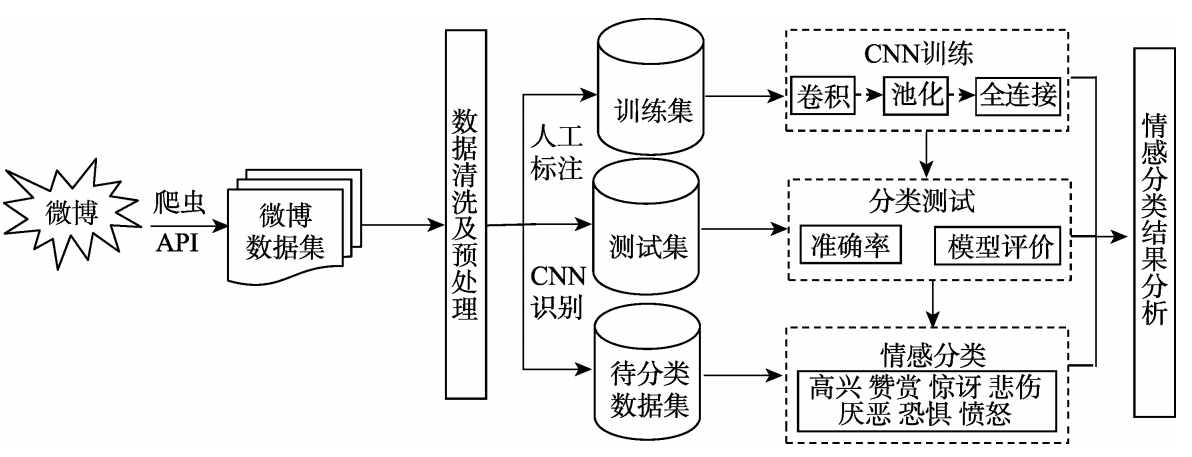
\includegraphics[width=0.8\textwidth]{img/zhang2018jiyu.png}
  \caption{基于卷积神经网络的微博情感分类模型,引自\cite{zhang2018jiyu}}
  \label{fig:zhang2018jiyu}
\end{figure}

张海涛等人\cite{zhang2018jiyu}则研究了中文微博和评论中的文本情感分类。他们针对当时微博上具一定争议性的话题\#打呼噜被室友群殴\#收集数据,确保了样本围绕同一个主题并且有充足的数据量。使用开源工具 NLPIR/ICTCLAS2016 对语料进行分词,再以词向量学习算法word2vec从语料中学习词的表示向量作为输入,以基于卷积神经网络的模型作为分类器,另外以支持向量机作为对照算法。实验结果显示在面向长文本的情感识别时,他们的系统比支持向量机性能更好,而面向短文本时则相反。

\section{存在的问题}

由于近年来各企业或机构对情感识别的需求增加,相关技术的研究备受关注,加上深度学习的快速发展,情感识别和反讽识别的性能水平也在逐年提升。然而相关研究依然存在一些问题需要深入探讨:

\begin{itemize}

\item {\bf 数据不均匀在多分类问题中的影响}。情感识别在早期以识别文本的正性、负性和中性情感为主,但随着应用场景越来越复杂,相关研究逐渐关注其中的细分类别,反讽识别等研究也如此。而在多分类问题中,各类别样本量分布不均匀一直是个备受关注的问题。因为在真实应用场景的多分类问题中,各个类别的样本量往往分布不均匀甚至差别很大,这会导致部分性能指标明显偏低。譬如在训练数据中样本量较少的类别在测试集上的召回率会明显比其他类别的低,间接拉低宏平均的召回率和F1值。然而目前主流的研究工作大部分只探索单个模型如何对多类别的数据进行建模,在人工神经网络领域则是不断提出新的网络结构以在整体上达得到更好的识别能力。另外也有透过数据增强的方法调整训练数据中样本的分布情况,但也难以针对个别类别的识别能力进行调整。

\item {\bf 在算法建模中引入上下文信息} 在一些场景下,仅凭一段文本的内容可能无法完全理解发言者想表达的内容,这在短文本的场景中尤其明显,如微博、评论等。为此目前一些研究会考虑引入文本的上下文,认为这些上下文中包含相关的信息,有助于理解原文的内容。但在不同场景下,上下文的类型不同,其对应建模方式也会有所不同。如在微博平台中,要对微博正文进行情感识别,那么可以引入微博底下的评论以定位该微博描述的事情,另一方面也可以引入用户过去发布的微博,对比他使用表情符的习惯和当前微博中使用的表情符来猜测用户想表达的情感。然而对于不同场景下不同类型的上下文,如何在算法建模中引入上下文信息始终没有一种通用的方法,对于具体的问题依然需要进行针对性的设计。

\end{itemize}

\section{本论文的内容安排}

本文针对上述的两个问题,提出了一种多分类器分层识别算法以及用于结合上下文的多通道分类模型,并分别基于两个应用场景进行实验以验证他们的有效性。本论文的内容安排如下。

第\ref{cha:problem_framework}章对面向文本的情感识别问题作出分析,给出一个统一的数学定义。然后我们会给出一个文本情感识别的研究框架,详细说明其中每一步完成的任务和目的。紧接着会介绍一些自然语言处理和情感识别的相关技术,对于后续实验用中使用到的技术,我们会给出相对充分的说明,另外也会给出相关技术的概要描述,以便于其他研究者在本论文未深入探索的方向进行拓展性的工作。

第\ref{cha:exp_irony_det}章针对面向微博的反讽识别提出了一种多分类器分层识别算法,同时引出一种针对多分类问题的算法设计框架。我们将基于国际比赛SemEval-2018的任务三\cite{van2018semeval}展开实验,其中包含两个子任务。子任务一为二分类问题,要求识别微博是否包含反讽的修辞手法。另一个子任务为四分类问题,数据与子任务一相同,但原本"反讽"一类的样本被细分成反讽的三个类型:基于相反语义的反讽、情景反讽、其他反讽。我们提出的多分类器分层识别算法面向子任务二的四分类问题,我们会首先对组成该算法的子模型进行分析,再对整个算法的最终识别结果和中间结果进行分析,以此验证算法的有效性以及其设计的合理性。最后进行错误分析,了解我们的算法在此研究问题中的不足之处。

在第\ref{cha:exp_context_emo}章,我们提出了一种多通道分类模型,用于结合在情感识别中起着不同作用的上下文信息。基于此多通道分类模型,我们再给出了一个和前一章的算法框架相似的多分类器分层情感识别算法,并应用于面向三轮对话的情感识别。我们将基于国际比赛SemEval-2019的任务三\cite{SemEval2019Task3}展开实验,该比赛要求参赛系统识别两人轮流发言的三轮对话中最后一轮发言者所表达的情感,其中一共涉及四个情感类别:高兴、悲伤、愤怒、其他。同样地,我们会对组成该算法的子模型进行分析,再对整个算法的最终识别结果和中间结果进行分析,一方面验证算法的有效性以及其设计的合理性,另一方面验证我们提出的多分类器分层识别算法框架在不同多分类问题上的通用性。

最后,第\ref{cha:conclusion}章将总结本篇论文中的主要贡献和实验结论,并根据前面各实验的错误分析为后续研究工作给出建议。












